\subsection{Descripción:}

Recibimos una red de servidores interconectados por enlaces, nos piden encontrar cual servidor debemos escoger como master (servidor que recibe los datos primero), de tal forma que se pueda actualizar la información en todos los sistemas en el menor tiempo posible.
Se sabe que se tarda el mismo tiempo de ir de servidor en servidor para todos los enlaces, y las copias dentro del mismo son instantáneas.
Además cada servidor transmite simultáneamente a todos los vecinos elegidos.

En resumen el proceso es:
\begin{itemize}
\item -Un servidor recibe la información por primera vez (master).
\item-Puede copiar instantáneamente la información para enviarla a todos los servidores con los que se conecta.
\item-Envía la información, y éstos la reciben al mismo tiempo, e inician el proceso de copiado para enviarlo a través de sus enlaces, y asi sucesivamente hasta que todos tengan su copia.
\end{itemize}
En el siguiente ejemplo vemos una red de servidores (nodos), y sobre cada uno la cantidad mínima de pasos que precisaría para copiar la información a ese servidor, tomando como master el nodo resaltado (A, B, C, D). Suponiendo que cada servidor copia a todos sus adyacentes en el momento en que recibe los datos.

\begin{center}
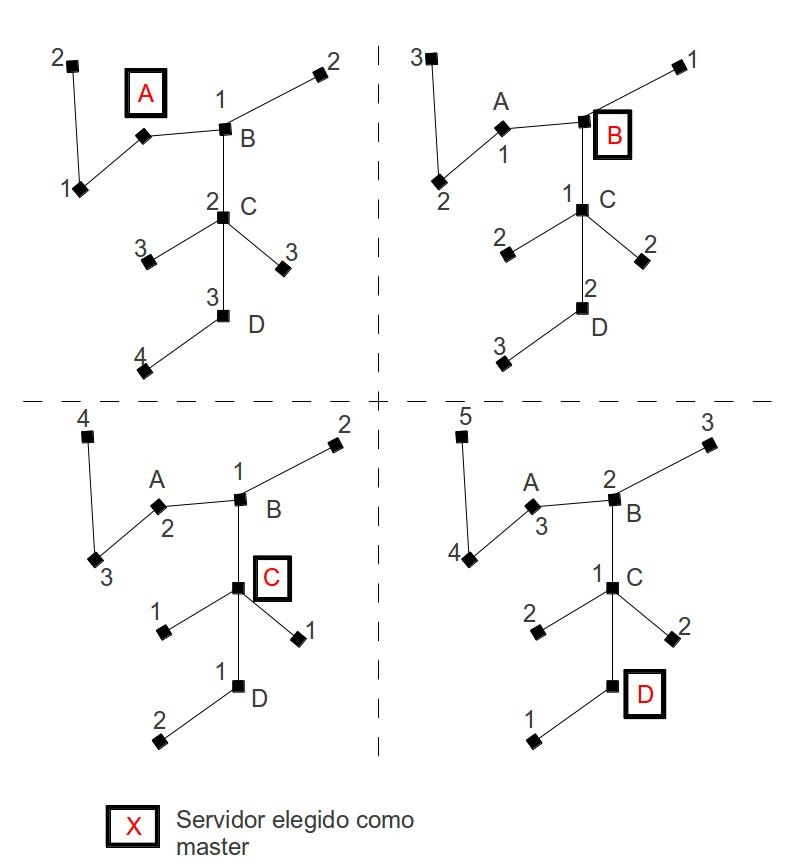
\includegraphics[scale=0.6]{ej2/2/graficos/imagen01.jpg} 
\end{center}

Vemos que si elegimos A o C, es posible completar la transferencia en 4 pasos, si elijo el D, en 5, y si escojo el B en sólo 3, por lo tanto este es nuestro "master"  óptimo (notar que se pueden tardar más pasos en completar todo, pero lo que queremos ver es la cantidad mínima).
En este caso la solución óptima fue una sola, pero pueden existir varias, un ejemplo sencillo es una red con sólo dos servidores conectados entre sí, podría poner a cualquiera como master.